
%%%%%%%%%%%%%%%%%%%%%%%%%%%%%%%%%%%%%%%%%%%%%%%%%%%%%%%%%%%%%%%%%%%%%%%%%%%%%
%
% intro.tex
%
% hamish, 6/8/1
%
% $Id: intro.tex,v 1.76 2006/09/28 00:03:52 niraj Exp $
%
%%%%%%%%%%%%%%%%%%%%%%%%%%%%%%%%%%%%%%%%%%%%%%%%%%%%%%%%%%%%%%%%%%%%%%%%%%%%%


%%%%%%%%%%%%%%%%%%%%%%%%%%%%%%%%%%%%%%%%%%%%%%%%%%%%%%%%%%%%%%%%%%%%%%%%%%%%%
\chapt[chap:intro]{Introduction}
\markboth{Introduction}{Introduction}
%%%%%%%%%%%%%%%%%%%%%%%%%%%%%%%%%%%%%%%%%%%%%%%%%%%%%%%%%%%%%%%%%%%%%%%%%%%%%
\nnormalsize
%%%% qqqqqqqqqqqqqqqqqqqqqqqqq %%%%
\ifprintedbook
\else
\begin{quote}
Software documentation is like sex:
when it is good, it is very, very good;
and when it is bad, it is better than nothing.
(Anonymous.)

There are two ways of constructing a software design: one way is
to make it so simple that there are obviously no
deficiencies; the other way is to make it so complicated that
there are no obvious deficiencies. (C.A.R. Hoare)

A computer language is not just a way of getting a computer to
perform operations but rather that it is a novel formal
medium for expressing ideas about methodology. Thus, programs
must be written for people to read, and only
incidentally for machines to execute.
(The Structure and Interpretation of Computer Programs, H. Abelson, G. Sussman
and J. Sussman, 1985.)

If you try to make something beautiful, it is often ugly.
If you try to make something useful, it is often beautiful.
(Oscar Wilde)\footnote{These were, at least, our ideals; of course we didn't
completely live up to them\ldots}
\end{quote}
\fi
%%%% qqqqqqqqqqqqqqqqqqqqqqqqq %%%%


%GATE is an infrastructure for developing and deploying software components
%that process human language. GATE helps scientists and developers in three
%ways:
%
%\begin{enumerate}
%
%\item
%by specifying an {\bf architecture}, or organisational structure, for
%language processing software;
%
%\item
%by providing a {\bf framework}, or class library, that implements the
%architecture and can be used to embed language processing capabilities in
%diverse applications;
%
%\item
%by providing a {\bf development environment} built on top of the
%framework made up of convenient graphical tools for developing components.
%\end{enumerate}
%
%The architecture exploits component-based software development, object
%orientation and mobile code. The framework and development environment are
%written in Java and available as open-source free software under the GNU
%library (or lesser) licence\footnote{This is a restricted form of the main GNU
%licence, which means that GATE can be embedded in commercial products if
%required.}. GATE uses Unicode throughout \cite{Uni96,Tablan02}, and has been 
%tested on a variety of Slavic, Germanic, Romance, and Indic languages
%\cite{May01,Gamback00,McE00}.
%
%From a scientific point-of-view, GATE's contribution is to
%quantitative measurement of accuracy and repeatability of results for
%verification purposes.
%
%GATE has been in development at the University of Sheffield since 1995 and has
%been used in a wide variety of research and development projects
%\cite{May00a}. Version 1 of GATE was released in 1996, was licensed by several
%hundred organisations, and used in a wide range of language analysis contexts
%including Information Extraction (\cite{Cun99c,App99,Gai98a,Cow96}) in
%English, Greek, Spanish, Swedish, German, Italian, French, Bulgarian, Russian,
%and a number of other languages. Version 4 of the system is available from
%\htlinkplain{http://gate.ac.uk/download/}.

GATE\footnote{If you've read
the overview at \htlinkplain{http://gate.ac.uk/overview.html}, 
you may prefer to skip to Section~\ref{sec:intro:howtouse}.} is an
infrastructure for developing and deploying software components that
process human language. It is nearly 15 years old and is in active use
for all types of computational task involving human language. GATE
excels at text analysis of all shapes and sizes. From large
corporations to small startups, from \texteuro multi-million research
consortia to undergraduate projects, our user community is the largest
and most diverse of any system of this type, and is spread across all
but one of the continents\footnote{Rumours that we're planning to send
several of the development team to Antarctica on one-way tickets are
false, libellous and wishful thinking.}.

GATE is open source \htlink{http://www.fsf.org/}{free software}; users
can obtain free support from the user and developer community
via \htlink{http://gate.ac.uk/}{GATE.ac.uk} or on a commercial basis
from \htlink{http://gate.ac.uk/customisation/}{our industrial partners}. We are the
biggest open source language processing project with a development
team more than double the size of the largest comparable projects
(many of which are integrated with GATE\footnote{Our philosophy is
reuse not reinvention, so we integrate and interoperate with other
systems\, e.g.: LingPipe, OpenNLP, UIMA, and many more specific
tools.}). More than \texteuro5 million has been invested in GATE
development\footnote{This is the figure for direct Sheffield-based
investment only and therefore an underestimate.}; our objective is to
make sure that this continues to be money well spent for all GATE's
users.

The GATE family of tools has grown over the years to include a desktop client for developers, a
workflow-based web application, a Java library, an architecture and a process.
GATE is:

\begin{itemize}
\item
\textit{an IDE}, \textbf{\htlink{http://gate.ac.uk/family/developer.html}{GATE Developer}}: 
  an integrated development environment\footnote{GATE
  Developer and GATE Embedded are bundled, and in older distributions were
  referred to just as `GATE'.} for
  language processing components bundled with a very widely used \htlink{http://gate.ac.uk/ie}{Information Extraction} system and a comprehensive set of
  \htlink{http://gate.ac.uk/gate/doc/plugins.html}{other plugins}
\item
\textit{a cloud computing solution} for hosted large-scale text
  processing, \textbf{GATE Cloud}
  (\htlinkplain{https://cloud.gate.ac.uk/}). See also Chapter~\ref{chap:cloud}.
\item
\textit{a web app}, \htlink{http://gate.ac.uk/teamware/}{\bf GATE Teamware}: a collaborative
  annotation environment for factory-style semantic annotation projects built
  around a workflow engine and a heavily-optimised backend service
  infrastructure. See also Chapter~\ref{chap:teamware}.
\item 
\textit{a multi-paradigm search repository}, \htlink{http://gate.ac.uk/family/mimir.html}{\bf GATE \Mimir},
 which can be used to index and search over text, annotations, semantic schemas
(ontologies), and semantic meta-data (instance data). It allows queries that
arbitrarily mix full-text, structural, linguistic and semantic queries and that
can scale to terabytes of text. See also Chapter~\ref{chap:mimir}.
\item
\textit{a framework}, \htlink{http://gate.ac.uk/family/embedded.html}{\bf GATE Embedded}: an object library
  optimised for inclusion in diverse applications giving access to all the
  services used by GATE Developer and more.
\item
\textit{an architecture}: a high-level organisational picture of how language
  processing software composition.
\item
\textit{a process} for the creation of \htlink{http://gate.ac.uk/family/process.html}{robust and
  maintainable services}.
\end{itemize}

We also develop:

\begin{itemize}
\item
a wiki/CMS, \textbf{GATE Wiki}
  (\htlinkplain{http://gatewiki.sf.net/}), mainly
  to host our own websites and as a testbed for some of our
  experiments
\end{itemize}

For more information on the GATE family see \htlinkplain{http://gate.ac.uk/family/} and also Part IV of this book.

One of our original motivations was to remove the necessity for
solving common engineering problems before doing useful research, or
re-engineering before deploying research results into
applications. Core functions of GATE take care of the lion's share of
the engineering:

\begin{itemize}
\item
modelling and persistence of specialised data structures
\item
measurement, evaluation, benchmarking (never believe a computing
    researcher who hasn't measured their results in a repeatable and open
    setting!)
\item
visualisation and editing of annotations, ontologies, parse trees, etc.
\item
a finite state transduction language for rapid prototyping and efficient
    implementation of shallow analysis methods (JAPE)
\item
extraction of training instances for machine learning
\item
pluggable machine learning implementations (Weka, SVM Light, ...)
\end{itemize}

On top of the core functions GATE includes components for diverse language
processing tasks, e.g. parsers, morphology, tagging, Information Retrieval tools,
Information Extraction components for various languages, and many others. GATE
Developer and Embedded are supplied with an Information Extraction system (ANNIE)
which has been adapted and evaluated very widely (numerous industrial systems,
research systems evaluated in MUC, TREC, ACE, DUC, Pascal, NTCIR, etc.). ANNIE is
often used to create RDF or OWL (metadata) for unstructured content
(\textit{\htlink{http://www.ontotext.com/kim/semanticannotation.html}{semantic
annotation}}).
  
GATE version 1 was written in the mid-1990s; at the turn of the new millennium we
completely rewrote the system in Java; version 5 was released in June 2009; and 
version 6 --- in November 2010. We
believe that GATE is the leading system of its type, but as scientists we have to
advise you not to take our word for it; that's why we've measured our software in
many of the competitive evaluations over the last decade-and-a-half (MUC, TREC,
ACE, DUC and more; see Section~\ref{sec:intro:evaluations} for details). We
invite you to give it a try, to get involved with the GATE community, and to contribute to
human language science, engineering and development.

This \thing\ describes how to use GATE to develop language processing
components, test their performance and deploy them as parts of other
applications. In the rest of this \chapthing:

\begin{itemize}
\item
Section \ref{sec:intro:howtouse} describes the best way to use this \thing;
\item
Section \ref{sec:intro:context} briefly notes that the context of GATE is
applied language processing, or {\em Language Engineering};
\item
Section \ref{sec:intro:overview} gives an overview of developing using GATE;
%\item
%section \ref{sec:structure} describes the structure of the rest of the \thing;
\item
Section \ref{sec:intro:evaluations} lists publications describing GATE
performance in evaluations;
\item
Section \ref{sec:intro:recent-changes} outlines what is new in the current
version of GATE;
\item
Section \ref{sec:intro:furtherreading} lists other publications about GATE.
\end{itemize}

Note: if you don't see the component you need in this document, or if we
mention a component that you can't see in the software, contact {\tt
gate-users@lists.sourceforge.net}\footnote{Follow the `support' link from
\htlinkplain{http://gate.ac.uk/} to subscribe to the mailing
list.} -- various components are developed by our collaborators, who
we will be happy to put you in contact with.  (Often the process of
getting a new component is as simple as typing the URL into GATE
Developer; the system will do the rest.)

%%%%%%%%%%%%%%%%%%%%%%%%%%%%%%%%%%%%%%%%%%%%%%%%%%%%%%%%%%%%%%%%%%%%%%%%%%%%
\sect[sec:intro:howtouse]{How to Use this Text}
%%%%%%%%%%%%%%%%%%%%%%%%%%%%%%%%%%%%%%%%%%%%%%%%%%%%%%%%%%%%%%%%%%%%%%%%%%%%

The material presented in this \thing\ ranges from the conceptual (e.g. `what is
software architecture?') to practical instructions for programmers (e.g. how to
deal with GATE exceptions) and linguists (e.g. how to write a pattern grammar).
Furthermore, GATE's highly extensible nature means that new functionality is
constantly being added in the form of new plugins. Important functionality is as
likely to be located in a plugin as it is to be integrated into the GATE core.
This presents something of an organisational challenge. Our (no doubt imperfect)
solution is to divide this \thing\ into three parts.
Part~\ref{part:intro-to-gate} covers installation, using the GATE Developer GUI
and using ANNIE, as well as providing some background and theory. We recommend
the new user to begin with Part~\ref{part:intro-to-gate}.
Part~\ref{part:advanced-gate} covers the more advanced of the core GATE
functionality; the GATE Embedded API and JAPE pattern language among other
things. Part~\ref{part:plugins} provides a reference for the numerous plugins
that have been created for GATE. Although ANNIE provides a good starting point,
the user will soon wish to explore other resources, and so will need to consult
this part of the text. We recommend that Part~\ref{part:plugins} be used as a
reference, to be dipped into as necessary. In Part~\ref{part:plugins}, plugins
are grouped into broad areas of functionality.

%It is a good idea to read all of this introduction (you can skip sections
%\ref{sec:context}, \ref{sec:evaluations} and \ref{sec:furtherreading} if
%pressed); then you can either continue wading through the whole thing or just
%use \chapthing\ \ref{chap:howto} as a reference and dip into other
%chapters for more detail as necessary. \Chapthing\
%\ref{chap:howto} gives instructions for completing common tasks with GATE,
%organised in a FAQ style: details, and the reasoning behind the various
%aspects of the system, are omitted in this \chapthing, so where more
%information is needed refer to later \chapthings.

%The structure of the
%\thing\ as a whole is detailed in section \ref{sec:structure} below.


%%%%%%%%%%%%%%%%%%%%%%%%%%%%%%%%%%%%%%%%%%%%%%%%%%%%%%%%%%%%%%%%%%%%%%%%%%%%
\sect[sec:intro:context]{Context}
%%%%%%%%%%%%%%%%%%%%%%%%%%%%%%%%%%%%%%%%%%%%%%%%%%%%%%%%%%%%%%%%%%%%%%%%%%%%

GATE can be thought of as a
\htlink{http://gate.ac.uk/sale/thesis/}{{\bf Software Architecture for
Language Engineering}} \cite{Cun00a}.

`Software Architecture' is used rather loosely here to mean
computer infrastructure for software development, including development
environments and frameworks, as well as the more usual use of the term to denote
a macro-level organisational structure for software systems \cite{Sha96a}.

Language Engineering (LE) may be defined as:
\begin{quote}
\ldots
the discipline or act of engineering software systems that perform tasks
involving processing human language. Both the construction process and its
outputs are measurable and predictable. The literature of the field relates
to both application of relevant scientific results and a body of
practice. \cite{Cun99b}
\end{quote}
The relevant scientific results in this case are the outputs of
Computational Linguistics, Natural Language Processing and Artificial
Intelligence in general. Unlike these other disciplines, LE, as an
engineering discipline, entails {\em predictability}, both of the process of
constructing LE-based software and of the performance of that software after
its completion and deployment in applications.

Some working definitions:

\begin{enumerate}
\item {\bf Computational Linguistics (CL):} science of language that uses
computation as an investigative tool.
\item
{\bf Natural Language Processing (NLP):} science of computation whose subject
matter is data structures and algorithms for computer processing of
human language.
\item
{\bf Language Engineering (LE):} building NLP systems whose cost and outputs
are measurable and predictable.
\item
{\bf Software Architecture:} macro-level organisational principles for
families of systems. In this context is also used as {\bf infrastructure}.
\item
{\bf Software Architecture for Language Engineering (SALE):}
software infrastructure, architecture and development tools for applied
CL, NLP and LE.
\end{enumerate}
%
(Of course the practice of these fields is broader and more complex than these
definitions.)

In the scientific endeavours of NLP and CL, GATE's role is to support
experimentation. In this context GATE's significant features include support
for automated measurement (see \Chapthing\ \ref{chap:eval}), providing a
`level playing field' where results can easily be repeated across different
sites and environments, and reducing research overheads in various ways.


%%%%%%%%%%%%%%%%%%%%%%%%%%%%%%%%%%%%%%%%%%%%%%%%%%%%%%%%%%%%%%%%%%%%%%%%%%%%
\sect[sec:intro:overview]{Overview}
%%%%%%%%%%%%%%%%%%%%%%%%%%%%%%%%%%%%%%%%%%%%%%%%%%%%%%%%%%%%%%%%%%%%%%%%%%%%


%%%%%%%%%%%%%%%%%%%%%%%%%%%%%%%%%%%%%%%%%%%%%%%%%%%%%%%%%%%%%%%%%%%%%%%%%%%%
\subsect[sec:intro:developing]{Developing and Deploying Language Processing
Facilities}
%%%%%%%%%%%%%%%%%%%%%%%%%%%%%%%%%%%%%%%%%%%%%%%%%%%%%%%%%%%%%%%%%%%%%%%%%%%%

GATE as an architecture suggests that the elements of software systems that
process natural language can usefully be broken down into various types of
component, known as resources\footnote{The terms `resource' and `component' are
synonymous in this context. `Resource' is used instead of just `component'
because it is a common term in the literature of the field: cf. the Language
Resources and Evaluation conference series \cite{Lrec98,Lrec00}.}. Components
are reusable software chunks with well-defined interfaces, and are a popular
architectural form, used in Sun's Java Beans and Microsoft's .Net, for
example. GATE components are specialised types of Java Bean, and come in
three flavours:
%
\begin{itemize}
%
\item
LanguageResources (LRs) represent entities such as lexicons, corpora or
ontologies;
%
\item
ProcessingResources (PRs) represent entities that are primarily algorithmic,
such as parsers, generators or ngram modellers;
%
\item
VisualResources (VRs) represent visualisation and editing components that
participate in GUIs.
%
\end{itemize}
%
These definitions can be blurred in practice as necessary.

Collectively, the set of resources integrated with GATE is known as
{\bf CREOLE}: a
Collection of REusable Objects for Language Engineering. All the resources are
packaged as Java Archive (or `JAR') files, plus some XML configuration data.
The JAR and XML files are made available to GATE by putting them on a web
server, or simply placing them in the local file space.
Section \ref{sec:intro:builtin-components} introduces GATE's built-in resource
set.

When using GATE to develop language processing functionality for an
application, the developer uses GATE Developer and GATE Embedded to
construct resources of the three types. This may involve programming,
or the development of Language Resources such as grammars that are
used by existing Processing Resources, or a mixture of both. GATE
Developer is used for visualisation of the data structures produced
and consumed during processing, and for debugging, performance
measurement and so on. For example, figure
\ref{fig:hindi} is a screenshot of one of the visualisation tools.
%
\begin{figure}[!htb]
\begin{center}
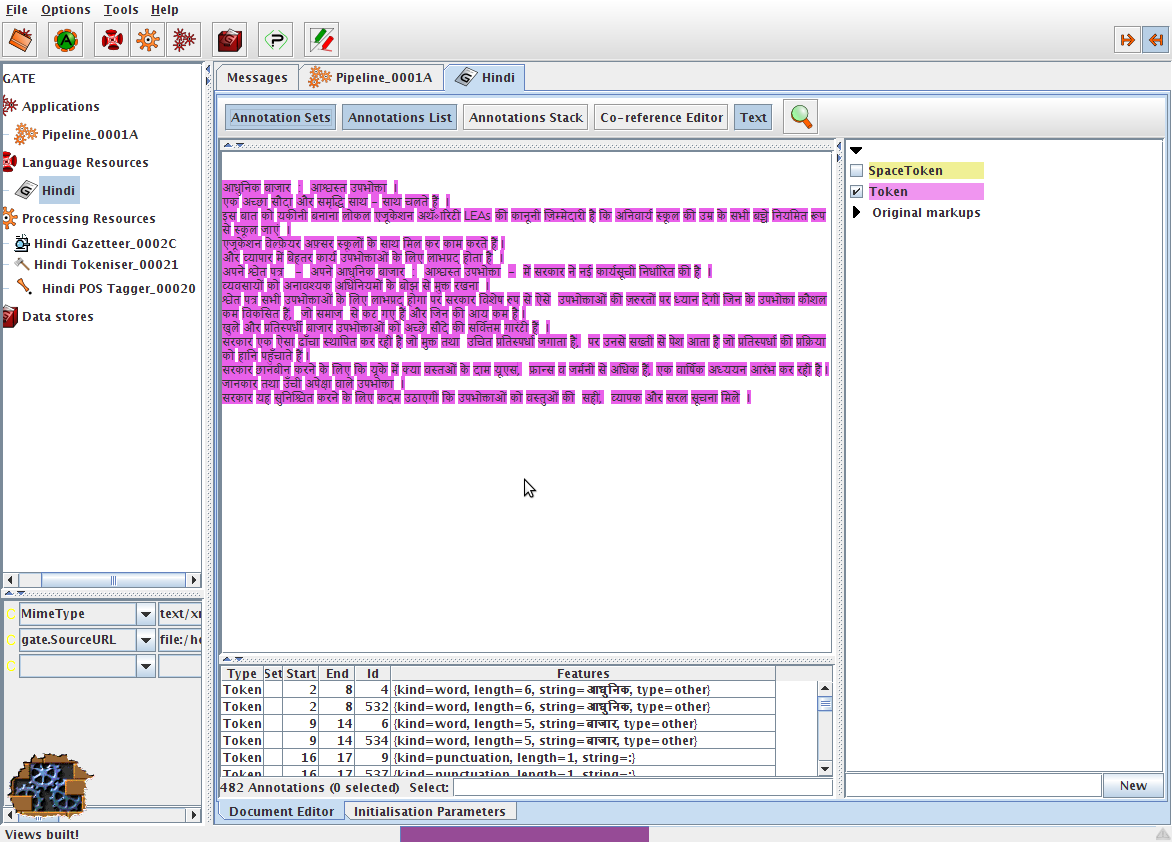
\includegraphics[width=14cm]{hindi-screenshot.png}
\end{center}
\caption{One of GATE's visual resources}
\label{fig:hindi}
\end{figure}
%
%(displaying named-entity extraction results for a Hindi sentence).

GATE Developer is analogous to systems like Mathematica for
Mathematicians, or JBuilder for Java programmers: it provides a
convenient graphical environment for research and development of
language processing software.

When an appropriate set of resources have been developed, they can then be
embedded in the target client application using GATE Embedded. GATE Embedded is
supplied as a series of JAR files.\footnote{The main JAR file ({\bf gate.jar})
supplies the framework. Built-in resources and various 3rd-party libraries are
supplied as separate JARs; for example ({\bf guk.jar}, the GATE Unicode Kit.)
contains Unicode support (e.g. additional input methods for languages not currently supported by the JDK). They
are separate because the latter has to be a Java extension with a privileged
security profile.} To embed GATE-based language processing facilities in an
application, these JAR files are all that is needed, along with JAR files and XML
configuration files for the various resources that make up the new facilities.


%%%%%%%%%%%%%%%%%%%%%%%%%%%%%%%%%%%%%%%%%%%%%%%%%%%%%%%%%%%%%%%%%%%%%%%%%%%%
\subsect[sec:intro:builtin-components]{Built-In Components}
%%%%%%%%%%%%%%%%%%%%%%%%%%%%%%%%%%%%%%%%%%%%%%%%%%%%%%%%%%%%%%%%%%%%%%%%%%%%

GATE includes resources for common LE data structures and algorithms,
including documents, corpora and various annotation types, a set of
language analysis components for Information Extraction and a range of data
visualisation and editing components.

GATE supports documents in a variety of formats including XML, RTF, email,
HTML, SGML and plain text. In all cases the format is analysed and converted
into a single unified model of {\em annotation}. The annotation format is
a modified form of the TIPSTER format \cite{Gri96b}
which has been made largely compatible with the Atlas format \cite{Bir99},
and uses the now standard mechanism of `stand-off markup'. GATE documents,
corpora and annotations are stored in databases of various sorts,
visualised via the
development environment, and accessed at code level via the framework.
See \Chapthing~\ref{chap:corpora} for more details of corpora etc.

A family of Processing Resources for language analysis is included in the
shape of ANNIE, A Nearly-New Information Extraction system. These components
use finite state techniques to implement various tasks from tokenisation to
semantic tagging or verb phrase chunking. All ANNIE components communicate
exclusively via GATE's document and annotation resources.
See \Chapthing~\ref{chap:annie} for more details. Other CREOLE resources are
described in Part~\ref{part:plugins}.


%%%%%%%%%%%%%%%%%%%%%%%%%%%%%%%%%%%%%%%%%%%%%%%%%%%%%%%%%%%%%%%%%%%%%%%%%%%%
\subsect[sec:intro:additional]{Additional Facilities in GATE Developer/Embedded}
%%%%%%%%%%%%%%%%%%%%%%%%%%%%%%%%%%%%%%%%%%%%%%%%%%%%%%%%%%%%%%%%%%%%%%%%%%%%

Three other facilities in GATE deserve special mention:
%
\begin{itemize}
%
\item
JAPE, a Java Annotation Patterns Engine, provides regular-expression based
pattern/action rules over annotations -- see \Chapthing~\ref{chap:jape}.
%
\item
The `annotation diff' tool in the development environment implements
performance metrics such as precision and recall for comparing annotations.
Typically a language analysis component developer will mark up some documents
by hand and then use these along with the diff tool to automatically measure
the performance of the components. See \Chapthing\ \ref{chap:eval}.
%
\item
GUK, the GATE Unicode Kit, fills in some of the gaps in the JDK's\footnote{JDK:
Java Development Kit, Sun Microsystem's Java implementation. Unicode support
is being actively improved by Sun, but at the time of writing many languages
are still unsupported. In fact, Unicode itself doesn't support all languages,
e.g. Sylheti; hopefully this will change in time.} support for
Unicode, e.g. by adding input methods for various languages from Urdu to
Chinese. See Section \ref{sec:developer:unicode} for more details.
\end{itemize}
%

%%%%%%%%%%%%%%%%%%%%%%%%%%%%%%%%%%%%%%%%%%%%%%%%%%%%%%%%%%%%%%%%%%%%%%%%%%%%
\subsect[sec:intro:example]{An Example}
%%%%%%%%%%%%%%%%%%%%%%%%%%%%%%%%%%%%%%%%%%%%%%%%%%%%%%%%%%%%%%%%%%%%%%%%%%%%

This section gives a very brief example of a typical use of GATE to develop
and deploy language processing capabilities in an application, and to
generate quantitative results for scientific publication.

Let's imagine that a developer called Fatima is building an email
client\footnote{Perhaps because
Outlook Express trashed her mail folder again, or because she got tired of
Microsoft-specific viruses and hadn't heard of Gmail or Thunderbird.} for
Cyberdyne Systems' large corporate Intranet.
In this application she would like to have a language processing system
that automatically spots the names of people in the corporation and
transforms them into {\tt mailto} hyperlinks.

A little investigation shows that GATE's existing components can be
tailored to this purpose. Fatima starts up GATE Developer, and creates
a new document containing some example emails. She then loads some
processing resources that will do named-entity recognition (a
tokeniser, gazetteer and semantic tagger), and creates an application
to run these components on the document in sequence. Having processed
the emails, she can see the results in one of several viewers for
annotations.

The GATE components are a decent start, but they need to be altered to
deal specially with people from Cyberdyne's personnel
database. Therefore Fatima creates new `cyber-' versions of the
gazetteer and semantic tagger resources, using the `bootstrap'
tool. This tool creates a directory structure on disk that has some
Java stub code, a Makefile and an XML configuration file.  After
several hours struggling with badly written documentation, Fatima
manages to compile the stubs and create a JAR file containing the new
resources. She tells GATE Developer the URL of these
files\footnote{While developing, she uses a {\tt file:/\ldots} URL;
for deployment she can put them on a web server.}, and the system then
allows her to load them in the same way that she loaded the built-in
resources earlier on.

Fatima then creates a second copy of the email document, and uses the annotation
editing facilities to mark up the results that she would like to see her system
producing. She saves this and the version that she ran GATE on into her serial
datastore. From now on she can follow this routine:
\begin{enumerate}
\item\label{item:run}
Run her application on the email test corpus.
\item
Check the performance of the system by running the `annotation diff' tool to
compare her manual results with the system's results. This gives her both
percentage accuracy figures and a graphical display of the differences
between the machine and human outputs.
\item
Make edits to the code, pattern grammars or gazetteer lists in her resources,
and recompile where necessary.
\item
Tell GATE Developer to re-initialise the resources.
\item
Go to \ref{item:run}.
\end{enumerate}
%
To make the alterations that she requires, Fatima re-implements the ANNIE
gazetteer so that it regenerates itself from the local personnel data.
She then alters the pattern grammar in the semantic tagger to prioritise
recognition of names from that source. This latter job involves learning the
JAPE language (see \Chapthing\ \ref{chap:jape}), but as this is based on
regular expressions it isn't too difficult.

Eventually the system is running nicely, and her accuracy is 93\%
(there are still some problem cases, e.g. when people use nicknames,
but the performance is good enough for production use). Now Fatima
stops using GATE Developer and works instead on embedding the new
components in her email application using GATE Embedded. This
application is written in Java, so embedding is very
easy\footnote{Languages other than Java require an additional
interface layer, such as JNI, the Java Native Interface, which is in
C.}: the GATE JAR files are added to the project CLASSPATH, the
new components are placed on a web server, and with a little code to
do initialisation, loading of components and so on, the job is
finished in half a day -- the code to talk to GATE takes up only
around 150 lines of the eventual application, most of which is just
copied from the example in the
\ifprintedbook
%This is because it's a huge overfull in the footnote, and I need to hyphenate that URL for the book
%to make it agree with the printers. But inserting the optional hyphenation point breaks the URL when not
%rendered as footnote in the book. Hence this solution, until somebody gets a better idea!
\htlink{http://gate.ac.uk/wiki/code-repository/javadoc/src-html/sheffield/examples/\-Stand\-Alone\-Annie.html}{{\small\tt sheffield.examples.StandAloneAnnie}} class.
\else
\htlink{http://gate.ac.uk/wiki/code-repository/javadoc/src-html/sheffield/examples/StandAloneAnnie.html}{{\small\tt sheffield.examples.StandAloneAnnie}} class.
\fi

Because Fatima is worried about Cyberdyne's unethical policy of developing
Skynet to help the large corporates of the West strengthen their
strangle-hold over the World, she wants to get a job as an academic instead
(so that her conscience will only have to cope with the torture of students,
as opposed to humanity). She takes the accuracy measures that she has
attained for her system and writes a paper for the Journal of Nasturtium
Logarithm Incitement describing the approach used and the results obtained.
Because she used GATE for development, she can cite the repeatability of her
experiments and offer access to example binary versions of her software by
putting them on an external web server.

And everybody lived happily ever after.


%%%%%%%%%%%%%%%%%%%%%%%%%%%%%%%%%%%%%%%%%%%%%%%%%%%%%%%%%%%%%%%%%%%%%%%%%%%%
%\sect[sec:structure]{Structure of the Book}
%%%%%%%%%%%%%%%%%%%%%%%%%%%%%%%%%%%%%%%%%%%%%%%%%%%%%%%%%%%%%%%%%%%%%%%%%%%%

%The material presented in this \thing\ ranges from the conceptual (e.g. `what
%is software architecture?') to practical instructions for programmers (e.g.
%how to deal with GATE exceptions) and linguists (e.g. how to write a pattern
%grammar). This diversity is something of an organisational challenge. Our (no
%doubt imperfect) solution is to collect specific instructions for `how to do
%X' in a separate \chapthing\ (\ref{chap:howto}). Other \chapthings\ give a
%more discursive presentation. In order to understand the whole system you
%must, unfortunately, read much of the \thing; in order to get help with a
%particular task, however, look first in \chapthing\ \ref{chap:howto} and
%refer to other material as necessary.
%
%The other \chapthings:
%
%\Chapthing\ \ref{chap:creole-model} describes the GATE architecture's
%component-based model of language processing, describes the lifecycle of GATE
%components, and how they can be grouped into applications and stored in
%databases and files.
%
%\Chapthing\ \ref{chap:gazetteers} describes the set of Visual Resources that are
% bundled with GATE.
%
%\Chapthing\ \ref{chap:corpora} describes GATE's model of document formats,
%annotated documents, annotation types, and corpora (sets of documents). It
%also covers GATE's facilities for reading and writing in the XML
%data interchange language.
%
%\Chapthing\ \ref{chap:jape} describes JAPE, a pattern/action rule language
%based on regular expressions over annotations on documents. JAPE grammars
%compile into cascaded finite state transducers.
%
%\Chapthing\ \ref{chap:annie} describes ANNIE, a pipelined Information
%Extraction system which is supplied with GATE.
%
%\Chapthing\ \ref{chap:ml} describes a machine learning layer specifically 
%targetted at NLP tasks including text classification, chunk learning 
%(e.g. for named entity recognition) and relation learning.
%
%\Chapthing\ \ref{chap:misc-creole} describes CREOLE resources
%bundled with the system that don't fit into the previous categories.
%
%\Chapthing\ \ref{chap:ontologies} describes processing resources and language
%resources for working with ontologies.
%
%\Chapthing\ \ref{sec:alignment} describes a plugin that allows users to
%create new tools for text alignment and cross-document processing.
%
%\Chapthing\ \ref{sec:eval} describes how to
%measure the performance of language analysis components.
%
%\Chapthing\ \ref{chap:api} describes programming using the GATE Embedded API.
%
%\Chapthing\ \ref{chap:security} describes the datastore security model.
%
%Appendix \ref{chap:design} discusses the design of the system.
%
%Appendix \ref{chap:japeimpl} describes the implementation details and
%formal definitions of the JAPE annotation patterns language.
%
%Appendix \ref{chap:negram} describes in some detail the JAPE pattern grammars
%that are used in ANNIE for named-entity recognition.


%%%%%%%%%%%%%%%%%%%%%%%%%%%%%%%%%%%%%%%%%%%%%%%%%%%%%%%%%%%%%%%%%%%%%%%%%%%%
\sect[sec:intro:evaluations]{Some Evaluations}
%%%%%%%%%%%%%%%%%%%%%%%%%%%%%%%%%%%%%%%%%%%%%%%%%%%%%%%%%%%%%%%%%%%%%%%%%%%%

This section contains an incomplete list of publications describing systems that
used GATE in competitive quantitative evaluation programmes. These programmes
have had a significant impact on the language processing field and the widespread
presence of GATE is some measure of the maturity of the system and of our
understanding of its likely performance on diverse text processing tasks.

%The University of Sheffield has a long history of research into
%open-domain question answering. GATE has formed the basis of much of this
%research resulting in systems which have ranked highly during independent
%evaluations since 1999. The first successful question answering system
%developed at the University of Sheffield was evaluated as part of TREC 8 and
%used the LaSIE information extraction system (the forerunner of ANNIE) which
%was distributed with GATE \cite{Humphreys99}. Further research was reported in
%\cite{Scott00}, \cite{Greenwood02}, \cite{Gaizauskas03a}, \cite{Gaizauskas04}
%and \cite{Gaizauskas05}. In 2004 the system was ranked 9th out of 28
%participating groups.

%Further publications documenting performance in evaluations include the
%following:

\begin{description}

\item[\cite{Yaoyong07b}] describes the performance of an SVM-based learning
system in the NTCIR-6 Patent Retrieval Task. The system achieved the best result
on two of three measures used in the task evaluation, namely the R-Precision and
F-measure. The system obtained close to the best result on the remaining measure
(A-Precision).

\item[\cite{Saggion'07a}] describes a cross-source coreference resolution system
based on semantic clustering. It uses GATE for information extraction and the 
SUMMA system to create summaries and semantic representations of documents. One
system configuration ranked 4th in the Web People Search 2007 evaluation.

\item[\cite{Saggion'06a}] describes a cross-lingual summarization system which
uses SUMMA components and the Arabic plugin available in GATE to produce
summaries in English from a mixture of English and Arabic documents.

\item[Open-Domain Question Answering:] The University of Sheffield has a long
history of research into open-domain question answering. GATE has formed the
basis of much of this research resulting in systems which have ranked highly
during independent evaluations since 1999. The first successful question
answering system developed at the University of Sheffield was evaluated as part
of TREC 8 and used the LaSIE information extraction system (the forerunner of
ANNIE) which was distributed with GATE \cite{Humphreys99}. Further research was
reported in
\cite{Scott00}, \cite{Greenwood02}, \cite{Gaizauskas03a}, \cite{Gaizauskas04}
and \cite{Gaizauskas05}. In 2004 the system was ranked 9th out of 28
participating groups.

\item[\cite{Saggion'04a}] describes techniques for answering definition
questions. The system uses definition patterns manually implemented in GATE as
well as learned JAPE patterns induced from a corpus. In 2004, the system was
ranked 4th in the TREC/QA evaluations.

\item[\cite{Saggion&Gaizauskas'04b}] describes a multidocument summarization
system implemented using summarization components compatible with GATE (the
SUMMA system). The system was ranked 2nd in the Document Understanding Evaluation
programmes.

\item[\cite{May03d} and \cite{May03g}] describe participation in the
TIDES surprise language program. ANNIE was adapted to Cebuano with four person days
of effort, and achieved an F-measure of 77.5\%. Unfortunately, ours was the only
system participating!

\item[\cite{Maynard02} and \cite{Maynard03}] describe results obtained on
systems designed for the ACE task (Automatic Content Extraction). Although a comparison
to other participating systems cannot be revealed due to the stipulations of ACE,
results show 82\%-86\% precision and recall.

\item[\cite{Hum98a}] describes the LaSIE-II system used in MUC-7.

\item[\cite{Gai95b}] describes the LaSIE-II system used in MUC-6.

\end{description}

%%%%%%%%%%%%%%%%%%%%%%%%%%%%%%%%%%%%%%%%%%%%%%%%%%%%%%%%%%%%%%%%%%%%%%%%%%%%
\sect[sec:intro:recent-changes]{Recent Changes}
%%%%%%%%%%%%%%%%%%%%%%%%%%%%%%%%%%%%%%%%%%%%%%%%%%%%%%%%%%%%%%%%%%%%%%%%%%%%

This section details recent changes made to GATE.
\ifprintedbook
  The complete changelog is available at \htlinkplain{http://gate.ac.uk/userguide/chap:changes\permalinktrailer}.
\else
  Appendix~\ref{chap:changes} provides a complete change log.
\fi

\nestedtrue

%'nested' switch is used to make section headings format correctly whether
%they are in the appendix or the introduction.
%
% Within this file you should use \rcSect[label]{Heading} instead of
% \sect[sec:changes:label]{Heading}, and \rcSubsect{Heading} instead of
% \subsect{Heading}.  These commands are redefined appropriately depending on
% whether we are processing the intro subsection or the full changelog
% appendix.
%
\ifnested
  \def\rcSectNoLabel#1{\subsect{#1}}
  \def\rcSect[#1]#2{\subsect[subsec:changes:#1]{#2}}
  \def\rcSubsect#1{\subsubsect{#1}}
  \def\rcSubsubsect#1{\subsubsubsect{#1}}
\else
  \def\rcSectNoLabel#1{\sect{#1}}
  \def\rcSect[#1]#2{\sect[sec:changes:#1]{#2}}
  \def\rcSubsect#1{\subsect{#1}}
  \def\rcSubsubsect#1{\subsubsect{#1}}
\fi

\rcSect[8.5.1]{Version 8.5.1 (June 2018)}

Version 8.5.1 is a minor release to fix a few critical bugs in 8.5:

\begin{itemize}
\item Fixed an exception that prevented the ANNIC search GUI from opening.
\item Fixed a problem with ``Export for GATE Cloud'' that meant some resources
  were not getting included in the output ZIP file.
\item Fixed the XML schema in the \verb!gate-spring! library.
\end{itemize}

\rcSect[8.5]{Version 8.5 (May 2018)}

GATE Developer and Embedded 8.5 introduces a number of significant internal
changes to the way plugins are managed, but with the exception of the plugin
manager most users will not see significant changes in the way they use GATE.

\begin{itemize}
\item The GATE plugins are no longer bundled with the GATE Developer
  distribution, instead each plugin is downloaded from a repository at runtime,
  the first time it is used.  This means the distribution is much smaller than
  previous versions.
\item Most plugins are now distributed as a single JAR file through the
  Java-standard ``Central Repository'', and resource files such as gazetteers
  and JAPE grammars are bundled inside the plugin JAR rather than being
  separate files on disk.  If you want to modify the resources of a plugin
  then GATE provides a tool to extract an editable copy of the files from
  a plugin onto your disk -- it is no longer possible to edit plugin grammars
  in place.
\item This makes dependencies between plugins much easier to manage -- a plugin
  can specify its dependencies declaratively by name and version number rather
  than by fragile relative paths between plugin directories.
\end{itemize}

GATE 8.5 remains backwards compatible with existing third-party plugins, though
we encourage you to convert your plugins to the new style where possible.

Further details on these changes can be found in sections
\ref{sec:developer:plugins} (the plugin manager in GATE Developer),
\ref{sec:api:plugins} (loading plugins via the GATE Embedded API),
\ref{sec:api:bootstrap} (creating a new plugin from scratch), and
\ref{sec:api:updateplugins} (converting an existing plugin to the new style).

If you have an existing saved application from GATE version 8.4.1 or earlier it
will be necessary to ``upgrade'' it to use the new core plugins.  An upgrade
tool is provided on the ``Tools'' menu of GATE Developer, and is described in
section Section~\ref{sec:developer:convertxgapp}.

\rcSubsect{For developers}

As part of this release, GATE development has moved from SourceForge to GitHub
-- bug reports, patches and feature requests should now use the GitHub issue
tracker as described in section~\ref{sec:development:bugs}.

% vim:ft=tex


\nestedfalse

%%%%%%%%%%%%%%%%%%%%%%%%%%%%%%%%%%%%%%%%%%%%%%%%%%%%%%%%%%%%%%%%%%%%%%%%%%%%
\sect[sec:intro:furtherreading]{Further Reading}
%%%%%%%%%%%%%%%%%%%%%%%%%%%%%%%%%%%%%%%%%%%%%%%%%%%%%%%%%%%%%%%%%%%%%%%%%%%%

Lots of documentation lives on 
\htlink{http://gate.ac.uk/}{the GATE web site}, including:
\begin{itemize}
\item \htlink{http://gate.ac.uk/demos/movies.html}{GATE online tutorials};

\item \htlink{http://gate.ac.uk/gate/doc/}{the main system
documentation tree};

\item \javadocroot{JavaDoc API documentation};

\item \htlink{https://github.com/GateNLP/gate-core}{source code (at GitHub)};
\end{itemize}

For more details about Sheffield University's work in human
language processing see
\htlink{http://nlp.shef.ac.uk/}{the NLP group pages}
or
\htlink{http://www.dcs.shef.ac.uk/\string ~hamish/LeIntro.html}{{\em A Definition and Short History of Language Engineering}} (\cite{Cun99b}).
For more details about Information Extraction see
\htlink{http://www.dcs.shef.ac.uk/\string ~hamish/IE/}{{\em IE, a User Guide}}
or the
\htlink{http://gate.ac.uk/ie/}{GATE IE pages}.

A list of publications on GATE and projects that use it (some of which are available on-line from
\htlink{http://gate.ac.uk/gate/doc/papers.html}{http://gate.ac.uk/gate/doc/papers.html}):

\textbf{2010}
%
\begin{description}

\item[\cite{Bontcheva2010a}] describes the Teamware web-based collaborative annotation environment, emphasising the different roles that users play in the corpus annotation process. 

\item[\cite{Damljanovic10}] presents the use of GATE in the development of controlled natural language interfaces. There is other related work by Damljanovic, Agatonovic, and Cunningham on using GATE to build natural language interfaces for quering ontologies. 

\item[\cite{Aswani10b}] discusses the use of GATE to process South Asian languages (Hindi and Gujarati). 

%
\end{description}

\textbf{2009}
%
\begin{description}

\item[\cite{Saggion09}] focuses in detail on the use of GATE for mining opinions and facts for business intelligence gathering from web content.

\item[\cite{Aswani09}] presents in more detail the text alignment component of GATE.

\item[\cite{Bontcheva09a}] is the `Human Language Technologies' chapter of `Semantic Knowledge Management' (John Davies, Marko Grobelnik and Dunja Mladenić eds.)

\item[\cite{DamljanovicAB09}] discusses the use of semantic annotation for software engineering, as part of the TAO research project.

\item[\cite{Laclavik09}] reviews the current state of the art in email processing and communication research, focusing on the roles played by email in information management, and commercial and research efforts to integrate a semantic-based approach to email.

\item[\cite{Yaoyong09a}] investigates two techniques
for making SVMs more suitable for language learning tasks. Firstly, an
SVM with uneven margins (SVMUM) is proposed to deal with the problem
of imbalanced training data.  Secondly, SVM active learning is
employed in order to alleviate the difficulty in obtaining labelled
training data. The algorithms are presented and evaluated on several
Information Extraction (IE) tasks.
 

\end{description}

\textbf{2008}
%
\begin{description}

\item[\cite{Agatonovic08}] presents our approach to automatic patent enrichment, tested in large-scale, parallel experiments on USPTO and EPO documents.

\item[\cite{DamljanovicTB08}] presents Question-based
Interface to Ontologies (QuestIO) - a tool for querying ontologies
using unconstrained language-based queries.

\item[\cite{DamljanovicB08a}] presents a semantic-based prototype that
is made for an open-source software engineering project with the goal
of exploring methods for assisting open-source developers and software
users to learn and maintain the system without major effort.


\item[\cite{DellaValle08}] presents ServiceFinder.

\item[\cite{Yaoyong08}] describes our SVM-based system and several techniques we developed successfully to adapt SVM for the specific features of the F-term patent classification task.

\item[\cite{Li08}] reviews the recent developments in applying geometric and quantum mechanics methods for information retrieval and natural language processing.

\item[\cite{Maynard08b}] investigates the state of the art in automatic textual annotation tools, and examines the extent to which they are ready for use
in the real world.

\item[\cite{Maynard08c}] discusses methods of measuring the performance of ontology-based information extraction systems, focusing particularly
on the Balanced Distance Metric (BDM), a new metric we have proposed
which aims to take into account the more flexible nature of
ontologically-based applications.
%
\item[\cite{Maynard07c}] investigates NLP techniques for ontology population, using a combination of rule-based approaches and machine learning.

\item[\cite{TablanDB08}] presents the QuestIO system – a natural language interface
for accessing structured information, that is domain independent and
easy to use without training.


\end{description}

\textbf{2007}
%
\begin{description}

\item[\cite{Funk07a}] describes an ontologically based approach to multi-source, multilingual information extraction.

\item[\cite{Funk07}] presents a controlled language for ontology editing and
a software implementation, based partly on standard NLP tools,
for processing that language and manipulating an ontology.

\item[\cite{Maynard07b}] proposes a methodology to capture (1) the evolution of metadata induced by changes to the
ontologies, and (2) the evolution of the ontology induced by changes
to the underlying metadata.

\item[\cite{Maynard07a}] describes the development of a
system for content mining using domain ontologies, which enables the
extraction of relevant information to be fed into models for analysis of
financial and operational risk and other business intelligence applications
such as company intelligence, by means of the XBRL standard.


\item[\cite{Saggion'07a}] describes experiments for the cross-document coreference task in SemEval 2007. Our cross-document coreference system uses an in-house agglomerative clustering implementation to group documents referring to the same entity.

\item[\cite{Saggion07}] describes the application of ontology-based extraction
and merging in the context of a practical e-business application for
the EU MUSING Project where the goal is to gather international
company intelligence and country/region information.


\item[\cite{Yaoyong07}] introduces a hierarchical learning approach for IE, which uses the target ontology as an essential part of the extraction process, by taking into account the relations between concepts.

\item[\cite{Yaoyong07a}] proposes some new evaluation measures based on relations among classification labels, which can be seen as the label relation sensitive version of important measures such as averaged precision and F-measure, and presents the results of applying the new evaluation measures to all submitted runs for the NTCIR-6 F-term patent classification task.

\item[\cite{Yaoyong07c}] describes the algorithms and linguistic features used in our participating system for the opinion analysis pilot task at NTCIR-6.

\item[\cite{Yaoyong07b}] describes our SVM-based system and the techniques we used to adapt the approach for the specifics of the F-term patent classification subtask at NTCIR-6 Patent Retrieval Task.

\item[\cite{Yaoyong07d}] studies Japanese-English cross-language patent retrieval using Kernel Canonical Correlation Analysis (KCCA), a method of correlating linear relationships between two variables in kernel defined feature spaces.

\end{description}

\textbf{2006}

\begin{description}

\item[\cite{Aswani06}] (Proceedings of the 5th International Semantic Web Conference (ISWC2006))
In this paper the problem of disambiguating author instances in
ontology is addressed. We describe a web-based approach that uses
various features such as publication titles, abstract, initials and
co-authorship information.

\item[\cite{Bon06a}] `Semantic Annotation and Human Language Technology', contribution to `Semantic Web Technology: Trends and Research' (Davies, Studer and Warren, eds.)


\item[\cite{Bon06b}] `Semantic Information Access', contribution to `Semantic Web Technology: Trends and Research' (Davies, Studer and Warren, eds.)

\item[\cite{Bon06c}] presents an ontology learning approach that 1) exploits a range of
information sources associated with software projects and 2) relies on
techniques that are portable across application domains.

\item[\cite{Dav06a}] describes work in progress concerning the application of Controlled Language
Information Extraction - CLIE to a Personal Semantic Wiki - Semper-
Wiki, the goal being to permit users who have no specialist knowledge
in ontology tools or languages to semi-automatically annotate their
respective personal Wiki pages.


\item[\cite{Yaoyong06a}] studies a machine learning algorithm based on KCCA for cross-language information retrieval. The algorithm is applied to Japanese-English cross-language information retrieval.

\item[\cite{Maynard06a}] discusses existing evaluation metrics, and proposes a new method for evaluating the ontology population task, which is general enough to be used in a variety of situation, yet more precise than many current metrics.

\item[\cite{Tablan06a}] describes an approach that allows users to create and edit ontologies simply by using a restricted version of the English language. The controlled language described
is based on an open vocabulary and a restricted set of grammatical
constructs.

\item[\cite{Tablan06b}] describes the creation of linguistic analysis and corpus search tools for Sumerian, as part of the development of the ETCSL.


\item[\cite{Wang06}] proposes an SVM based approach
to hierarchical relation extraction, using features derived
automatically from a number of GATE-based open-source language
processing tools.


\end{description}

\textbf{2005}

\begin{description}

\item[\cite{Aswani05}] (Proceedings of Fifth International Conference on Recent Advances in Natural Language Processing (RANLP2005))
It is a full-featured annotation indexing and search engine, developed
as a part of the GATE. It is powered with Apache Lucene technology and
indexes a variety of documents supported by the GATE.

\item[\cite{Bon05a}] presents the ONTOSUM system which uses Natural Language Generation (NLG) techniques to produce textual summaries from Semantic Web ontologies.

\item[\cite{Cun05a}] is an overview of the field of Information Extraction
for the 2nd Edition of the Encyclopaedia of Language and Linguistics.
%
\item[\cite{Cun05b}] is an overview of the field of Software Architecture
for Language Engineering
for the 2nd Edition of the Encyclopaedia of Language and Linguistics.
%
\item[\cite{DowmanEtAl05b}] (Euro Interactive Television Conference Paper)
A system which can use material from the Internet to augment television news broadcasts.
%
\item[\cite{DowmanEtAl05a}] (World Wide Web Conference Paper)
The Web is used to assist the annotation and indexing of broadcast news.
%
\item[\cite{DowmanEtAl05c}] (Second European Semantic Web Conference Paper)
A system that semantically annotates television news broadcasts using
news websites as a resource to aid in the annotation process.
%
\item[\cite{Yaoyong05}] (Proceedings of Sheffield Machine Learning Workshop)
describe an SVM based IE system which uses the SVM with uneven margins
as learning component and the GATE as NLP processing module.
%
\item[\cite{Yaoyong05a}] (Proceedings of Ninth Conference on Computational Natural Language Learning (CoNLL-2005))
uses the uneven margins versions of two popular learning algorithms SVM and Perceptron for IE to 
deal with the imbalanced classification problems derived from IE. 

\item[\cite{Yaoyong05b}] (Proceedings of Fourth SIGHAN Workshop on Chinese Language processing (Sighan-05))
a system for Chinese word segmentation based on Perceptron learning, a
simple, fast and effective learning algorithm.

\item[\cite{Polajnar05}] (University of Sheffield-Research Memorandum CS-05-10) User-Friendly Ontology Authoring Using a Controlled Language.

\item[\cite{Saggion&Gaizauskas'05a}] describes experiments on content selection for producing biographical summaries from multiple documents.

\item[\cite{Ursu05}] (Proceedings of the 2nd European Workshop on the Integration of Knowledge, Semantic and Digital Media Technologies (EWIMT 2005))Digital Media Preservation and Access through Semantically Enhanced Web-Annotation.

\item[\cite{Wang05}] (Proceedings of the 2005 IEEE/WIC/ACM International Conference on Web Intelligence (WI 2005)) Extracting a Domain Ontology from Linguistic Resource Based on Relatedness Measurements.

\end{description}

\textbf{2004}

\begin{description}

\item[\cite{Bon04a}] (LREC 2004) describes lexical and ontological resources
in GATE used for Natural Language Generation.
%
\item[\cite{Bon04b}] (JNLE) discusses developments in GATE in the early
naughties.
%
\item[\cite{Cun04b}] (JNLE) is the introduction to the above collection.
%
\item[\cite{Cun04a}] (JNLE) is a collection of papers covering many
important areas of Software Architecture for Language Engineering.
%
\item[\cite{Dim04a}] (Anaphora Processing) gives a lightweight method for
named entity coreference resolution.
%
\item[\cite{Yaoyong04}] (Machine Learning Workshop 2004)
describes an SVM based learning algorithm for IE using GATE.
%
\item[\cite{May04a}] (LREC 2004) presents algorithms for the automatic
induction of gazetteer lists from multi-language data.
%
\item[\cite{May04c}] (ESWS 2004) discusses ontology-based IE in the
hTechSight project.
%
\item[\cite{May04b}]  (AIMSA 2004) presents automatic creation and
monitoring of semantic metadata in a dynamic knowledge portal.
%
\item[\cite{Saggion&Gaizauskas'04}] describes an approach to mining definitions.

\item[\cite{Saggion&Gaizauskas'04b}] describes a sentence extraction system that produces two sorts of multi-document summaries; a general-purpose summary of a cluster of related documents and an entity-based summary of documents related to a particular person.


\item[\cite{Wood04a}] (NLDB 2004) looks at ontology-based IE from parallel
texts.
%
\end{description}

\textbf{2003}

\begin{description}

\item[\cite{Bon03a}] (NLPXML-2003) looks at GATE for the semantic web.
%
\item[\cite{Cun03a}] (Corpus Linguistics 2003) describes GATE as a tool for
collaborative corpus annotation.
%
\item[\cite{Kir03}] (Technical Report) discusses semantic web technology in
the context of multimedia indexing and search.
%
\item[\cite{Manov03}] (HLT-NAACL 2003) describes experiments with
geographic knowledge for IE.
%
\item[\cite{Maynard03a}] (EACL 2003) looks at the distinction between
information and content extraction.
%
\item[\cite{May03e}] (Recent Advances in Natural Language Processing 2003)
looks at semantics and named-entity extraction.
%
\item[\cite{May03d}] (ACL Workshop 2003) describes NE extraction without
training data on a language you don't speak (!).
%
\item[\cite{Saggion03c}] (EACL 2003) discusses robust, generic and
query-based summarisation.
%
\item[\cite{Saggion&al03}] (Data and Knowledge Engineering) discusses
multimedia indexing and search from multisource multilingual data.
%
\item[\cite{Saggion03b}] (EACL 2003) discusses event co-reference in the
MUMIS project.
%
\item[\cite{Tab03a}] (HLT-NAACL 2003) presents the OLLIE on-line learning
for IE system.
%
\item[\cite{Wood03}] (Recent Advances in Natural Language Processing 2003)
discusses using parallel texts to improve IE recall.
%
\end{description}

\textbf{2002}

\begin{description}

\item[\cite{McE02}] (LREC 2002)
report results from the EMILLE Indic languages corpus collection and
processing project.
%
\item[\cite{Bon02d}] (ACl 2002 Workshop)
describes how GATE can be used as an environment for teaching NLP,
with examples of and ideas for future student projects developed
within GATE.
%
\item[\cite{Bon02a}] (NLIS 2002)
discusses how GATE can be used to create HLT modules for use in information
systems.

\item[\cite{Bon02c}, \cite{Dim02a} and \cite{Dimitrov02}]
(TALN 2002, DAARC 2002, MSc thesis)
describe the shallow named entity coreference modules in GATE:
the orthomatcher which resolves pronominal coreference,
and the pronoun resolution module.
%
\item[\cite{Cun01b}] (Computers and the Humanities)
describes the philosophy and motivation behind the system, describes GATE
version 1 and how well it lived up to its design brief.
%
\item[\cite{Cun02b}] (ACL 2002)
describes the GATE framework and graphical development environment as a
tool for robust NLP applications.

\item[\cite{Dim02a,Dimitrov02b}] (DAARC 2002, MSc thesis) discuss
lightweight coreference methods.
%
\item[\cite{Lal02a}] (Master Thesis) looks at text summarisation using GATE.
%
\item[\cite{Lal02b}] (ACL 2002) looks at text summarisation using GATE.
%
\item[\cite{May02e}] (ACL 2002 Summarisation Workshop)
describes using GATE to build a portable IE-based summarisation system
in the domain of health and safety.
%
\item[\cite{May02b}] (AIMSA 2002)
describes the adaptation of the core ANNIE modules within GATE to the ACE
(Automatic Content Extraction) tasks.

\item[\cite{May02d}] (Nordic Language Technology)
describes various Named Entity recognition projects developed at Sheffield
using GATE.
%
\item[\cite{May02a}] (JNLE)
describes robustness and predictability in LE systems, and presents
GATE as an example of a system which contributes to robustness and to
low overhead systems development.
%
\item[\cite{Pastra02}] (LREC 2002)
discusses the feasibility of grammar reuse in applications using ANNIE modules.
%
\item[\cite{Saggion02} and \cite{Saggion&al2002b}] (LREC 2002, SPLPT 2002)
describes how ANNIE modules have been adapted to extract information for
indexing multimedia material.
%
\item[\cite{Tablan02}] (LREC 2002)
describes GATE's enhanced Unicode support.
%
\end{description}

\ifprintedbook 
\else
\textbf{Older than 2002}

\begin{description}

\item[\cite{May01}] (RANLP 2001)
discusses a project using ANNIE for named-entity recognition across wide
varieties of text type and genre.
%
\item[\cite{Bon00a} and \cite{Bru99a}] (COLING 2000, technical report)
describe a prototype of GATE version 2 that integrated with the
\htlink{http://www.mpi.nl/world/tg/lapp/eudico/eudico.html}{EUDICO
multimedia markup tool} from the Max Planck Institute.
%
\item[\cite{Cun00a}] (PhD thesis)
defines the field of Software Architecture for Language Engineering,
reviews previous work in the area, presents a requirements analysis for such
systems (which was used as the basis for designing GATE versions 2 and 3),
and evaluates the strengths and weaknesses of GATE version 1.
%
\item[\cite{Cun00d}, \cite{Cun98a} and \cite{Pet98a}]
(OntoLex\linebreak 2000, LREC 1998)
presents GATE's model of Language Resources, their access and distribution.
%
\item[\cite{Cun00b}] (LREC 2000)
taxonomises Language Engineering components and discusses the requirements
analysis for GATE version 2.
%
\item[\cite{Cun00c} and \cite{Cun99a}] (COLING 2000, AISB 1999)
summarise experiences with GATE version 1.
%
\item[\cite{Cun00e} and \cite{Cun99d}] (technical reports)
document early versions of JAPE (superseded by the present document).
%
\item[\cite{Gamback00}] (LREC 2000)
discusses experiences in the Svensk project, which used GATE version 1
to develop a reusable toolbox of Swedish language processing components.
%
\item[\cite{May00a}] (technical report)
surveys users of GATE up to mid-2000.
%
\item[\cite{McE00}] (Vivek)
presents the
\htlink{http://www.emille.lancs.ac.uk/}{EMILLE project}
in the context of which
GATE's Unicode support for Indic languages has been developed.
%
\item[\cite{Cun99b}] (JNLE)
reviewed and synthesised definitions of Language Engineering.
%
\item[\cite{Ste98} and \cite{Cun98}] (ECAI 1998, NeMLaP 1998)
report work on implementing a word sense tagger in GATE version 1.
%
\item[\cite{Cun97a}] (ANLP 1997)
presents motivation for GATE and GATE-like infrastructural systems for
Language Engineering.
%
\item[\cite{Cun96g}] (manual)
was the guide to developing CREOLE components for GATE version 1.
%
\item[\cite{Cun96h}] (TIPSTER)
discusses a selection of projects in Sheffield using GATE version 1 and the
TIPSTER architecture it implemented.
%
\item[\cite{Cun96b,Cun96,Cun95}] (COLING 1996, AISB Workshop 1996,
technical report) report early work on GATE version 1.
%
\item[\cite{Gai96d}] (manual)
was the user guide for GATE version 1.
%
\item[\cite{Gai96b,Cun97e,Cun96c}] (ICTAI \linebreak 1996, TIPSTER 1997, NeMLaP 1996)
report work on GATE version 1.
%
\item[\cite{Hum96}] (manual)
describes the language processing components distributed with GATE version 1.
%
\item[\cite{Cun94a,Cun94}] (NeMLaP 1994, technical report)
argue that software engineering issues such as reuse, and framework
construction, are important for language processing R\&D.
%
\end{description}
%
\fi
